
\section{Introduction}

\begin{figure}[t]
\centering
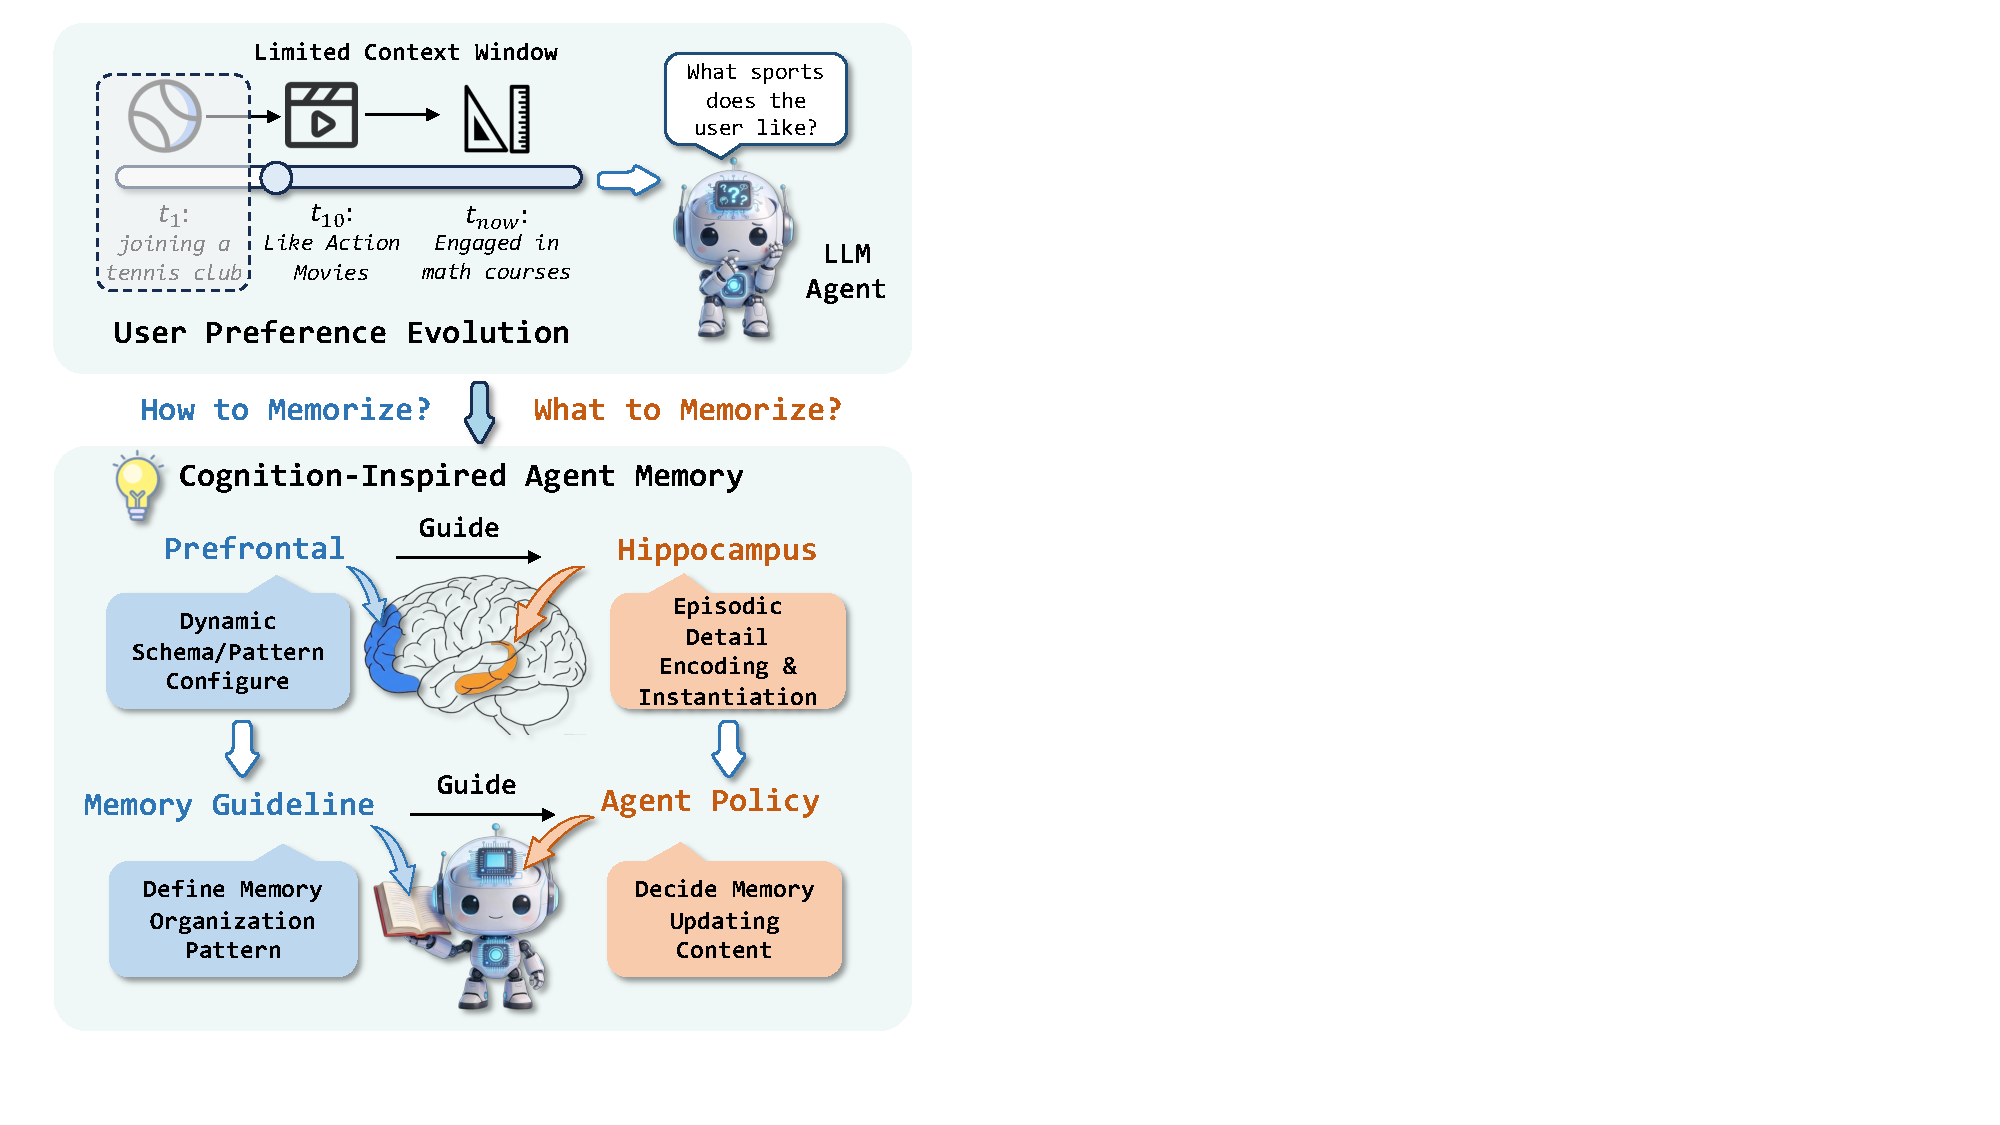
\includegraphics[width=0.99\columnwidth]{img/intro.pdf}
\caption{ Top: With a limited context window, the agent fails to capture preferences. Bottom: Inspired by \textcolor{PrefrontalBlue}{\textbf{\texttt{Prefrontal}}} $\rightarrow$ \textcolor{HippoOrange}{\textbf{\texttt{Hippocampus}}}, we decouple agent memory into \textcolor{PrefrontalBlue}{\textbf{\texttt{Memory Guideline}}} (for organizing) $\rightarrow$ \textcolor{HippoOrange}{\textbf{\texttt{Agent Memory}}} (for updating).}
\label{fig:intro}
\end{figure}

Large language models (LLMs) have demonstrated remarkable capabilities as conversational agents in various real-world applications, such as personal assistant \cite{li2024personalsurvey}, customer service \cite{RMM,zhang2025notellm}, and education \cite{AI4EDU}.
In these settings, adaptive personalized interaction depends on the agent's ability to continuously integrate information about a user’s evolving preferences and habits \cite{personamem,jiang2025personamemv2}.
However, the context window prevents LLMs from retaining and exploiting the full history of dialogue \cite{parallelencoding}, and simply storing and retrieving past dialogue snippets struggles to capture such dynamic patterns \cite{li2025memos}.
This limitation highlights the necessity of maintaining an external memory that preserves important information over time, enabling consistent and personalized responses \cite{chhikara2025mem0,memorybank,deng2026enhancing}.

Many existing LLM agent memory systems typically build a workflow that converts raw dialogue into external memory banks \cite{xu2026from,xu2025amem,fang2025lightmem}. Yet these methods rely on static and predefined pipelines for extraction rules, making it difficult to learn from interaction feedback or adapt to user behavior. To solve this, other works treat memory operations as learnable actions and train an end-to-end memory update policy with reinforcement learning (RL) \cite{yu2025memagent,memory-r1,wang2025memalpha}. While more adaptive, memory updates typically involve free-form edits over what to write or forget. When guided by only simple instructions and optimized with sparse and delayed outcome-level rewards, the policy is weakly constrained and faces a large action space, making exploration and long-horizon optimization challenging. This often results in unstable training and increased data requirements \cite{agentrlsurvey}, motivating the need for more effective mechanisms for memory organization and updating.


Memory schema theory \cite{alba1983memoryschematic} in cognitive psychology, as shown in Figure~\ref{fig:intro} bottom, offers a perspective for understanding how human memory is organized and updated. Specifically, the theory suggests a functional division of labor between brain systems: \textbf{Prefrontal regions} dynamically select and configure an appropriate schema based on the current context, thereby shaping expectations and attentional priorities, while the \textbf{Hippocampus regions} \cite{teyler1986hippocampal} instantiate this schema by encoding the concrete episodic details of ongoing experience. 
Importantly, this division is advantageous because it maintains a \textbf{stable schema-level organizing prior} that guides attention and structuring, while allowing the hippocampus system to flexibly encode context-specific episodic details within that scaffold. From this perspective, the separation naturally decouples how memory is controlled (i.e., the organization patterns) and what is stored (i.e., the update content).
Motivated by this mechanism, we ask the following question:
\definecolor{cvprblue}{rgb}{0.21,0.49,0.74}
\begin{tcolorbox}[colframe=black!50, colback=cvprblue!8, boxrule=1.5pt, arc=2mm, top=4pt, bottom=4pt, left=4pt, right=4pt,  boxsep=1pt]
\raisebox{-0.2\baselineskip}{
\includegraphics[height=1\baselineskip]{img/icon.png}}
\textit{Can we build a schema-based agent memory system whose organization and updating mechanisms evolve in a manner analogous to human brain?}
\end{tcolorbox}

To answer this question, in this paper, we introduce \ourmodel, a two-stage optimization framework inspired by a functional analogy to human memory, enabling the agent to learn \textbf{\texttt{how}} memory should be organized, and \textbf{\texttt{what}} content should be stored and updated, by optimizing a memory guideline and a policy for evolving memory. Our approach maintains a user memory bank that evolves alongside the dialogue. In the first stage, to simulate the Prefrontal regions, we propose $\clubsuit\ $\textbf{Memory Guideline Induction (MGI)}, which treats the instruction prompt as a global natural-language parameter and optimizes it via two key techniques: (i) interpreting contrastive feedback over memory-augmented trajectories as textual gradients and (ii) aggregating these gradients at the batch level, thereby inducing a domain-agnostic textual guideline. In the second stage, we propose $\spadesuit\ $\textbf{Guideline-Aligned Memory Policy Optimization (GMPO)}, which encodes instance-specific episodic details via guideline-aligned policy optimization. GMPO utilizes the optimized guideline to define guideline-aligned rewards and performs multi-turn RL over memory-augmented trajectories to train the memory-evolution policy end-to-end, thereby jointly encouraging adherence to the guideline and determining what content should be memorized. Crucially, the first stage induces a guideline that defines a stable set of memory operations, effectively constraining the action space explored by the policy. Given this constrained space, the second stage can focus on process-level guideline reward, learning to invoke the guideline-specified operations with appropriate content.


We empirically evaluate \ourmodel on three personalization memory benchmarks (PersonaMem, PrefEval, and PersonaBench), spanning explicit and implicit preference and increasingly noisy evidence sources, where accurate answering requires tracking evolving user states over extended histories. Across these settings, \ourmodel consistently outperforms strong baselines built on static memory templates or RL-based memory updating, while remaining \textbf{efficient} in memory evolution and \textbf{scalable} to longer contexts and more rounds. Moreover, the induced guideline exhibits strong \textbf{transferability} across LLMs, supporting \textbf{robust generalization} under distribution shifts in query type.

% Ablations further demonstrate that (i) learning the memory guideline via textual gradients is essential for transferring the memory system across domains and annotation styles, and (ii) reinforcement learning on top of the induced guideline effectively adapts the agent to complex, non-stationary user behaviors. Together, these results suggest that explicitly separating \emph{how} and \emph{what} agents memorize is a promising direction for building LLM-based assistants capable of reliable, long-term personalization.

